
\section{Experiments}
\label{sec:Experiments}






\subsection{For at least three different classifiers, systematically vary the most important hyperparameters and answer the following questions for each of them: }
\label{sec:Experiments:a}

The chosen classifier are \textbf{Random Forest, SVM and Logistic Regression}.

\begin{enumerate}[label=\roman*.)]
\item \textbf{How does classification performance change with varying hyperparameter values? Visualize the
change in performance.}

For tuning the hyperparameters 5\% of the training set was used on different combinations of hyperparameters.

\textbf{Random Forest} \quad
To find the optimal hyperparameters for Random Forest, different combinations of n\_estimators, max\_depth and min\_samples\_split were tested (See table \ref{tab:Tested hyperparameters}). Overall, the performance is  unsatisfactory and especially bad with low max\_depth values (See figure\ref{fig:F1 Score for different hyperparameters (Random Forest)}.

\textbf{SVM} \quad
To find the optimal hyperparameters for SVM, different combinations of C and kernel  were tested (See table \ref{tab:Tested hyperparameters}). More extensive testing was not feasible due to the long training times. SVM performs relatively good and the result of the testing is that low C values on the rbf kernel lead to the best results (See figure \ref{fig:F1 Score for different hyperparameters (SVM)}).


\textbf{Logistic Regression} \quad

To find the optimal hyperparameters for Logistic Regression, different combinations of C, penalty and solver  were tested (See table \ref{tab:Tested hyperparameters}). The performance iscomparable with SVM but the training time is many times faster. The only outlier was the combination of l2 and newton-cholesky which yielded very long training durations (See figure \ref{fig:F1 Score for different hyperparameters (Logistic Regression)}).
\begin{table}[htbp]
    \centering
    \begin{tabular}{cccccccc}\toprule
         \multicolumn{3}{c}{Tested hyperparameters (Random Forest} & \multicolumn{2}{c}{Tested hyperparameters (SVM)}& \multicolumn{3}{c}{Tested hyperparameters (Logistic Regression)}\\\midrule
         n\_estimators&  max\_depth& min\_samples\_split & C& kernel
& C& penalty&solver
\\
         10&  5& 2 & 0.1& linear
& 0.001& l2&lbfgs
\\
         30&  10& 5 & 1& rbf
& 0.01& None&newton-cholesky
\\
         50&  None& 10 & 10& poly& 0.1& &
\\ \bottomrule
    \end{tabular}
    \caption{Tested hyperparameters}
    \label{tab:Tested hyperparameters}
\end{table}


\begin{figure}[h]
  \centering
  \begin{minipage}[b]{0.49\textwidth}
    \centering
    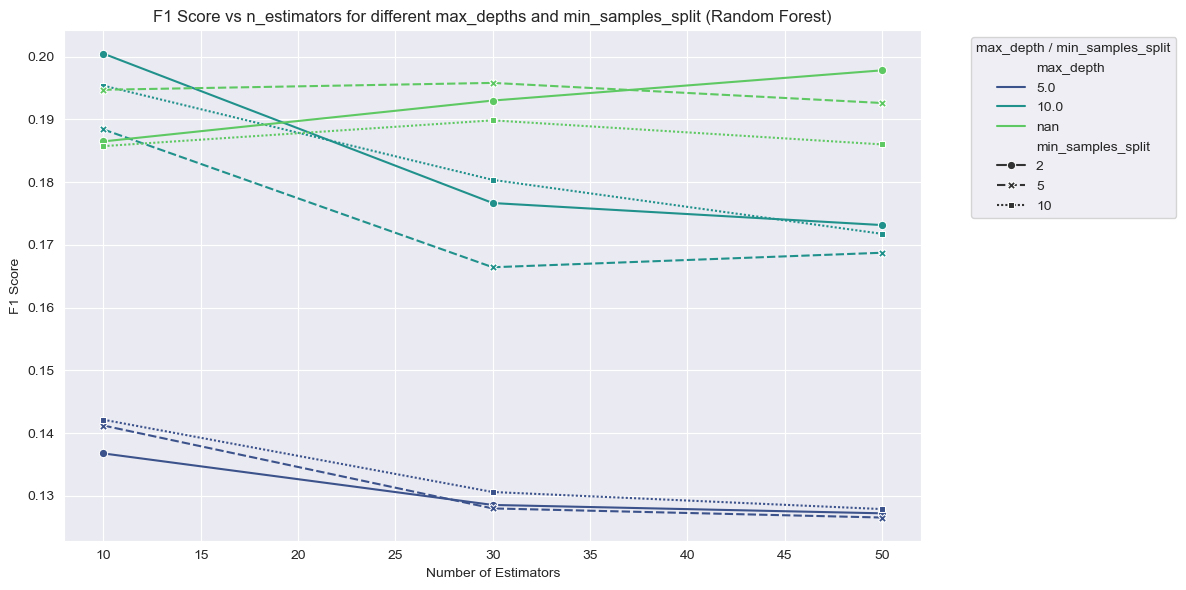
\includegraphics[width=\textwidth]{figs/Random_Forest.png}
    \caption{F1 Score for different hyperparameters (Random Forest)}
    \label{fig:F1 Score for different hyperparameters - Random Forest}
  \end{minipage}
  \hfill
  \begin{minipage}[b]{0.49\textwidth}
    \centering
    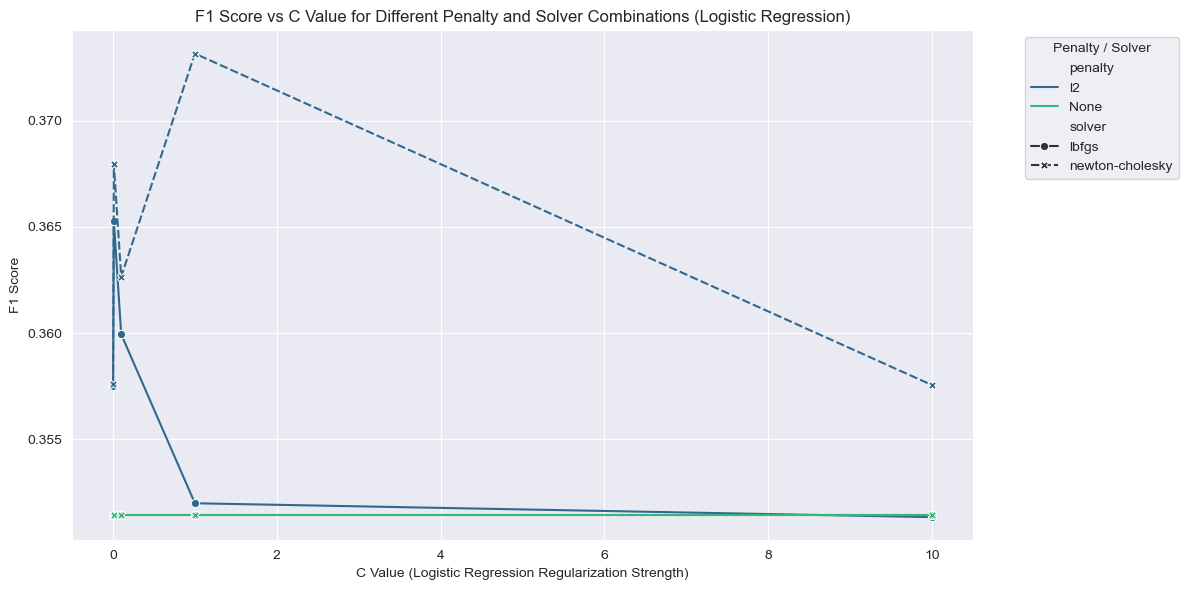
\includegraphics[width=\textwidth]{figs/Logistic_Regression.png}
    \caption{F1 Score for different hyperparameters (Logistic Regression)}
    \label{fig:F1 Score for different hyperparameters - Logistic Regression}
  \end{minipage}
\end{figure}

\begin{figure}[htbp]
    \centering
    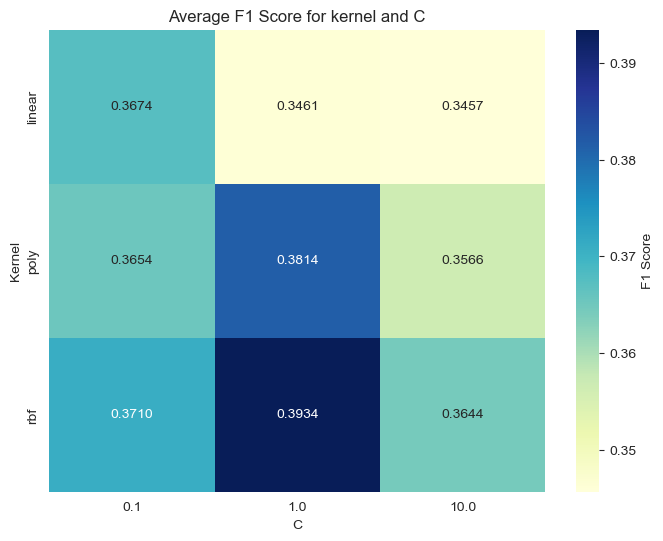
\includegraphics[width=0.5\linewidth, height=5cm]{figs/SVM.png}
    \caption{F1 Score for different hyperparameters (SVM)}
    \label{fig:F1 Score for different hyperparameters - SVM}
\end{figure}

\item \textbf{(To what extent) Does overfitting or underfitting occur, and what does it depend on?}
\end{enumerate}

\textbf{Random Forest} \quad
n\_estimators: Severe underfitting for  n\_estimators = 10. Severe overfitting for n\_estimators $\geq$ 30
max\_depth: Strong underfitting for max\_depth = 5.
min\_samples\_split: Dependent of the max\_depth, but doesn't cause major changes to the performance.

\textbf{SVM} \quad
C and kernel:  For rbf and polynomial kernal, minor underfitting can be detected at C < 1( See figure \ref{fig:F1 Score for different hyperparameters (SVM)}). Overfitting occurs for rbf and polynomial kernel at C $\geq$ 1 and for the linear kernel at C > 1.

\textbf{Logistic Regression} \quad
No major signs of over- or underfitting were observed

\subsection{After selecting appropriate hyperparameters, compare the final performance estimate of the three classifiers. }
\label{sec:Experiments:b}

The used hyperparameters and amount of training data used for the final models are dependent on the performance and train times during the parameter tuning:\\
Random Forest: n\_estimators=10; max\_depth=10; min\_samples\_split=5; 30\% of the training set was used.\\
SVM: C=1; kernel=rbf; 25\% of the training set was used.\\
Logistic Regression: C=0.1; penalty=l2; solver=lbfgs; 100\% of the training set was used.\\

The final results are as expected Logistic Regression > SVM > Random Forest (See table \ref{tab:Final Model Evaluation})
\begin{table}[htbp]
    \centering
    \begin{tabular}{ccccccccc}\toprule
         \multicolumn{3}{c}{Random Forest}&  \multicolumn{3}{c}{SVM}&  \multicolumn{3}{c}{Logistic Regression}\\\midrule
         F1 Score&  Accuracy&  Training Time&  F1 Score&  Accuracy&  Training Time&  F1 Score&  Accuracy& Training Time\\
         0.3217&  0.6174&  2409s&  0.4565&  0.7236&  17754s&  0.5460&  0.7587& 6487s\\ \bottomrule
    \end{tabular}
    \caption{Final Model Evaluation}
    \label{tab:Final Model Evaluation}
\end{table}
